\documentclass[a4paper,ngerman]{scrartcl}

\usepackage[utf8]{inputenc}
\usepackage[ngerman]{babel}
\usepackage{amsmath,amsthm,amssymb,amscd,color,graphicx,environ}
\usepackage{framed}
\usepackage[protrusion=true,expansion=true]{microtype}
\usepackage{lmodern}
\usepackage{multicol}
\usepackage[normalem]{ulem}
\usepackage{hyperref}

\usepackage{geometry}
\geometry{tmargin=1.5cm,bmargin=4cm,lmargin=3cm,rmargin=3cm}

\setlength{\unitlength}{1cm}

\setlength\parskip{\medskipamount}
\setlength\parindent{0pt}

\renewcommand*\theenumi{\alph{enumi}}
\renewcommand{\labelenumi}{\theenumi)}

\newlength{\aufgabenskip}
\setlength{\aufgabenskip}{1.4em}
\newcounter{aufgabennummer}
\newenvironment{aufgabe}[1]{
  \addtocounter{aufgabennummer}{1}
  \textbf{Aufgabe \theaufgabennummer.} \emph{#1} \par
}{\vspace{\aufgabenskip}}
\newenvironment{aufgabeE}[1]{\begin{aufgabe}{#1}\begin{enumerate}}{\end{enumerate}\end{aufgabe}}

\clubpenalty=10000
\widowpenalty=10000
\displaywidowpenalty=10000

\newcommand{\NN}{\mathbb{N}}
\newcommand{\RR}{\mathbb{R}}

\begin{document}

Institut für Mathematik \\
Universität Augsburg

\begin{center}
  \textbf{Übungsblatt zur Vorlesung} \\
  \emph{Geheimnis der Zahl 5}
\end{center}
\vspace{1em}

\begin{aufgabe}{Ein Kästchen verschwindet!}
\begin{enumerate}
\item Die beiden Figuren bestehen offensichtlich aus denselben Stücken, haben
aber unterschiedlichen Flächeninhalt! Was ist hier passiert?
\item Zeige: Der Quotient zweier aufeinanderfolgender Fibonacci-Zahlen nähert
sich beliebig genau dem goldenen Schnitt an.
\end{enumerate}
\begin{center}
  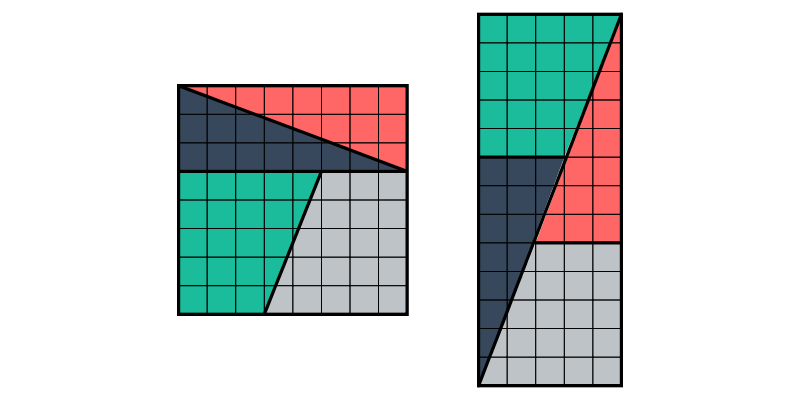
\includegraphics[scale=0.3]{ein-kaestchen-verschwindet}
\end{center}
\end{aufgabe}

\begin{aufgabe}{Die Quadrate der Fibonacci-Zahlen}
Es gilt die Identität~$\sum_{i=0}^n f_i^2 = f_n f_{n+1}$.
\begin{enumerate}
\item Führe einen Induktionsbeweis.
\item Argumentiere, wieso folgende Skizze die Behauptung auch schon beweist.
\end{enumerate}
\begin{center}
  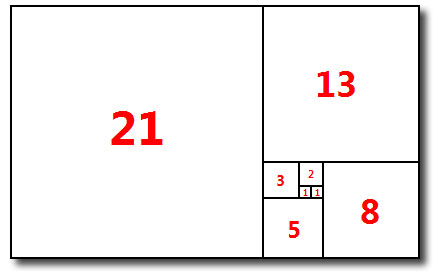
\includegraphics[scale=0.3]{fibonacci-quadrate}
\end{center}
\end{aufgabe}

\begin{aufgabe}{Irrationalste Zahl}
Formuliere präzise und beweise: Der goldene Schnitt ist die irrationalste Zahl.

\emph{Tipp:} Kettenbruchentwicklung.
\end{aufgabe}

\begin{aufgabe}{Ableitung vs. Umkehrfunktion}
Finde eine bijektive differenzierbare Funktion~$\RR^+ \to \RR^+$, deren
Ableitung gleich ihrer Umkehrfunktion ist.
\end{aufgabe}

\begin{aufgabe}{Conways Armee}
Ein unendlich ausgedehntes Damebrett sei in zwei Hälften zerteilt. Im unteren
Teil darf man beliebig viele Damesteine platzieren. Ziel des Spiels ist es,
einen Damestein möglichst hoch in das obere Spielfeld zu
bringen. Dabei darf nur folgender Spielzug angewendet werden: Ein Stein
darf einen (horizontal oder vertikal) benachbarten Stein überspringen, wenn das
Zielfeld unbesetzt ist. Der übersprungene Stein wird dann aus dem Spiel
entfernt.
\begin{enumerate}
\item Überzeuge dich davon, dass man, um Höhe~1, 2, 3 bzw. 4 über der
Trennlinie zu erreichen, mit~2, 4, 8 bzw. \sout{16} 20 Steinen beginnen muss.
\item Zeige, dass Höhe~5 mit keiner endlichen Anzahl von Steinen erreichbar
ist.

\emph{Tipp:} Weise den Spielsteinen eine von der Manhattan-Entfernung zum
angepeilten Zielstein abhängige Bewertung zu.
\end{enumerate}
\end{aufgabe}

\begin{aufgabe}{Auflösbarkeit quintischer Gleichungen}
Zeige, dass Gleichungen vom Grad~5 und höher im Allgemeinen nicht durch
Radikale auflösbar sind.

\emph{Tipp:} Eine Gleichung ist genau dann durch Radikale auflösbar, wenn die
zugehörige Galoisgruppe eine auflösbare Gruppe ist. Wenn man daher zeigt, dass
die symmetrische Gruppe in~$n$ Ziffern für $n \geq 5$ nicht auflösbar ist, hat
man schon viel gewonnen.
\end{aufgabe}

\begin{aufgabe}{Eine Zahl mit besonderer Dezimalbruchentwicklung}
Es gilt:
\[ \frac{1}{998999} =
  0{,}000\,001\,001\,002\,003\,005\,008\,013\,021\ldots. \]
\begin{enumerate}
\item Was ist daran besonders?
\item Inwiefern setzt sich das Muster auch nach~$987$ fort?
\item Erkläre das Phänomen.
\end{enumerate}
\end{aufgabe}

\begin{aufgabe}{Willmore-Satz}
Kathrin und Meru, ihr seid gefragt!
\end{aufgabe}

\begin{aufgabe}{Ein Lemma über goldene Dreiecke}
\begin{enumerate}
\item Zeige: In einem gleichschenkligen Dreieck mit den
Innenwinkeln~$72^\circ$, $36^\circ$ und~$72^\circ$ teilen die langen Seiten die
Grundseite im goldenen Schnitt.
\item Beweise damit folgende Pentagon-Dekagon-Hexagon-Identität: Seien ein
reguläres Pentagon, ein reguläres Dekagon und ein reguläres Hexagon in einem
Kreis einbeschrieben. Dann gilt für die Kantenlängen~$P$,~$D$ bzw.~$H$ die
Identität $P^2 = D^2 + H^2$.
\end{enumerate}
\end{aufgabe}

\begin{aufgabe}{Ein naiver Algorithmus für Fibonacci-Zahlen}
Eine ganz naive Methode, die~$n$-te Fibonacci-Zahl zu bestimmen, besteht
darin, die beiden Vorgänger zu bestimmen und dann zu summieren. Wie viele
Rechenschritte sind dabei notwendig, wenn man sich \emph{nicht}
Zwischenergebnisse merkt und daher viele Fibonacci-Zahlen immer wieder
berechnet?
\end{aufgabe}

\vfill

Noch zu \TeX{}en:
\begin{itemize}
\item \url{http://math.ucr.edu/home/baez/six.html}
\item \url{http://en.wikipedia.org/wiki/Wythoff%27s_game}
\item Beweise: $\sum_{i=0}^n F_i^2 = F_n F_{n+1}$ graphisch, und zwar mit der
Skizze aus
\url{http://math.stackexchange.com/questions/733754/visually-stunning-math-concepts-which-are-easy-to-explain}.
\item \url{https://www.math.hmc.edu/~benjamin/papers/DIE.pdf}, Seite 4, oben:
kombinatorische Interpretation der Fibonacci-Zahlen
\item Simons Aufgaben:
\url{github.com/NicolasMalebranche/Latex/tree/master/JHE%20S%C3%A4tze}
\end{itemize}

Bis Ende des Sommersemesters zu erledigen:
\begin{itemize}
\item Tolles Layout überlegen: Je zwei Seitenlängen müssen im goldenen Schnitt
zueinander stehen. Das jetzige Layout ist fast ungeändert von seinen eigenen
Übungsblättern übernommen.
\item Viele weitere kanonische und unkanonische Aufgaben finden.
\item Darauf achten, dass die Gesamtzahl von Aufgaben eine Fibonacci-Zahl ist.
\end{itemize}

\end{document}
